\documentclass{ciit-dissertation}

\usepackage{amsmath}
\usepackage{amsfonts}
\usepackage{caption}
\usepackage{verbatim}
\usepackage{fancyvrb}
\usepackage{graphicx}


\addbibresource{thesis.bib}


% Declare all of the data required to create the frontmatter (title pages, declarations .etc)
\title{Beam Forming With Phased Array Antennas}
\author{Laaraib}
\registrationnumber{CIIT/SP14-BPH-024/ISB}
\department{Physics}
\campus{Islamabad}
\degreetype{\undergraduate}
\program{BS Physics}
\dissertationtype{Thesis}
\session{Fall 2017}
\submissiondate{Jan 2, 2018}

\supervisor{Dr. Abid H. Mujtaba}
\supervisordesignation{Assistant Professor}

\hod{Dr. Sajid Qamar}
\hoddesignation{Professor}

\externalexaminer{}
\externalexaminerdesignation{}
\externalexaminerinstitution{}
\externalexamineraddress{Islamabad}

\dedication{I Dedicate My Thesis To My Dear Parents, Mr. and Mrs. Muhammad Mansha.}

\acknowledgement{After all the struggles and hard work of a complete year, now is the time that I pay my gratitude to the people responsible for making this possible for me.
	
First and foremost, I owe a great debt of gratitude to My supervisor "Dr. Abid Mujtaba", for the continuous support of My project work and related research, for his patience, motivation and immense knowledge. Without his assistance and dedicated involvement in every step throughout the process, this thesis would have never been accomplished. Thank you sir, for your sage advices and vital guidance, which made it possible to complete My project and writing of this thesis.

Most importantly, I am deeply grateful to My Parents and Siblings, for their attention, support and being there for me throughout My life.
		
		Thank you!}

\abstract{To create a high gain antenna, which radiates radio waves in a narrow beam, two general techniques can be used;
	
One technique is to use large metal surfaces such as parabolic reflectors, horns or dielectric lenses which change the direction of the radio waves by reflection or refraction, to focus the radio waves from a single low gain antenna into a beam. This type is called an aperture antenna.
	
And second technique, is to use multiple antennas to form a directed beam (beam forming) which involves the operations of phase shifting and amplitude tapering for each element, this is called phased array antenna, or antenna array. Depending upon their geometry we have different configuration of arrays for e.g linear, circular and complex array.
	
By using the second technique, My task was to construct the plot between intensity and lateral distance, for multiple antenna sources arranged in a linear array and by managing only the phase between them to produce a directed beam (one with maximum intensity at a location of my choice).}

\begin{document}
	
	\makefrontmatter        % Create all of the pages before the first chapter: title, dedication, ack, abstract, ToC, LoF .etc
	
    \chapter{Introduction}

A person, who needs to convey a thought or an idea can do so by voice communication, which takes place through sound waves. However, if two people want to communicate who are at longer distances, then we have to convert these sound waves into electromagnetic waves. The device, which converts the required information signal into electromagnetic waves, is known as an Antenna.\\
Now what if we are dealing with signals at very large distances as they are very faint with low frequencies like cosmic signals. Radio Telescopes are used for this purpose which consist of large dish antennas because large diameters are require to resolve radio sources at low frequencies and longer wavelengths so a large collecting area is needed to detect the signals at very large distances.\\
The infeasibility of constructing such large antenna dishes and the demand for higher resolution and sensitivity led us to the development of interferometric techniques which involve the use of multiple smaller antennae to get more reliable results instead of using a large setup which is hard to build up due to mechanical limitations.\\
To overcome the problem of signal efficiency at large distances we use an array of antennas to effectively synthesize a large aperture with an increased sensitivity and resolution.
 

\section{Maxwell's Equations}

Maxwell’s equations are a set of partial differential equations for the electric and magnetic fields as functions of space and time, that together with the Lorentz force law, form the foundation of classical electromagnetism, Quantum field theory, Classical optics, and electric circuits.\\ 
Following are the well known Maxwell's equations.

\begin{enumerate}
   \item Gauss’ Law For Electrostatics

      Electric charge produces an electric field, and the flux of that field passing through any closed surface is proportional to the total charge contained within that surface.\\
      \begin{equation}
      \vec{\nabla}.\vec{E} = \frac{\rho_{enc}}{\epsilon_{o}}
      \end{equation}

   \item Gauss’s Law For Magnetism

   There are no magnetic monopoles. The total magnetic flux through a closed surface is zero.\\
   \begin{equation}
   \vec{\nabla}.\vec{B} = 0
   \end{equation}

   \item Faraday’s Law Of Induction

   The voltage induced in a closed circuit is proportional to the rate of change of the magnetic flux.\\
   \begin{equation}
   \vec{\nabla}\times\vec{E} = - \frac{\partial\vec{B}}{\partial t}
   \end{equation}

   \item Ampere’s Law

      The magnetic field induced around a closed loop is proportional to the electric current.\\
      \begin{equation}
      \vec{\nabla}\times\vec{B} =\mu_{o}\vec{J}
      \end{equation}
      and with the Maxwell's correction Ampere's law becomes\\
      \begin{equation}
      \vec{\nabla}\times\vec{B} =\mu_{o}\vec{J}+\mu_{o}\epsilon_{o}\frac{\partial\vec{E}}{\partial t}
      \end{equation}
      where\\

      $\epsilon_{o}\frac{\partial\vec{E}}{\partial t}\equiv$ Displacement Current

\end{enumerate}

\section{Antennas and Beam Forming}

\subsection{Isotropic Antenna}
Antenna is a specialized transducer that converts radio frequency into alternating current or vice versa, and as antenna patterns are the same while transmitting or receiving, thus receiving end works the same as the transmitting end.\\
There are several different types of antennas and they all have their place. One of them is an isotropic antenna.\\
Isotropic antenna is an ideal antenna that radiates its power uniformly in all directions over a sphere centered on the source, and we get the same intensity of radiation in all directions.

\subsection{Beam Forming}
When a signal is sent out it gets wider and wider there-by losing its strength. Therefore we need a technique to focus signals.\\
Beam forming is a technique use to combine signals from an array of antennas to effectively synthesize a single aperture and beam, to simulate a large directional antenna.\\
It is achieved by combining signals from antennas in an array with right delay and phase, in such a way that signals at particular angles experience constructive interference while others experience destructive interference, and we get a directive beam.\\
Beam forming is considered as a subset of smart antennas or Advanced Antenna Systems (AAS), which typically exploit the properties of multiple antennas operating together.\\
To get stronger beam forming effect we will add more antennas in the array.

\subsection{Phased Array}
A phased array is composed of lots of radiating elements with a correct phase relationship so that the multiple transmitted patterns combine in the transmitting media by natural coherence of these radiations, and form a “beam”, a signal targeted to the destination.\\
By this way, The phases overlap and amplify each other and in the desired direction (where the destined receiver is located) and where the beam is not supposed to go the phases collide and destroy each other.\\
We can change the directionality of the beam by controlling the phase and relative amplitude of the signal at each transmitter. So by phased arrays we can steer the main beam of the antennas without physically moving the antenna.\\
Depending upon their geometry we have different configuration of arrays:

\begin{enumerate}

   \item Simple Arrays
      \begin{enumerate}

         \item Linear

            Antenna elements arranged along a straight line.

         \item Planar

            Antenna elements arranged over some planar surfaces.

      \end{enumerate}

   \item Complex Arrays

      Design by placing elements on certain specific position to get desirable beam. In general there are two types of phased arrays:

      \begin{enumerate}

         \item Passive Phased Array

            In which the antenna elements are connected to a single transmitter and receiver.

         \item Active Phased Array

            In which each antenna element has its own transmitter and receiver.Active arrays are more advanced.

      \end{enumerate}

\end{enumerate}

\section{Scope of the Project}

This project analyzed a directive beam created by a linear array of multiple antennas by signal spacing among them. 
To achieve this, I used Python to compare the expected simulated outcomes to theoretical results (which were calculated using Maxwell's Equation and the Electromagnetic Wave Equation).

    \chapter{Isotropic Propagation of Electromagnetic Waves}

\section{Maxwell's Equations in Vacuum}

As in vacuum charge density $\rho$ and current density $\vec{j}$ vanishes, so Maxwell's equations become:

\begin{enumerate}

   \item Gauss’s Law For Electricity

      \begin{equation}\label{gauss_law}
      \vec{\nabla}.\vec{E} = 0
      \end{equation}

   \item Gauss’s Law For Magnetism

      \begin{equation}
      \vec{\nabla}.\vec{B} = 0
      \end{equation}

   \item Faraday’s Law Of Induction

      \begin{equation}\label{faraday_induction}
      \vec{\nabla}\times\vec{E} = - \frac{\partial\vec{B}}{\partial t}
      \end{equation}

   \item Ampere’s Law

      \begin{equation}\label{amperes_law}
      \vec{\nabla}\times\vec{B} = \mu_{o}\epsilon_{o}\frac{\partial\vec{E}}{\partial t}
      \end{equation}

\end{enumerate}

Now if we apply curl to \eqref{faraday_induction}
%
   \begin{equation}\label{curl_of_induction}
   \vec{\nabla}\times(\vec{\nabla}\times\vec{E}) = - \vec{\nabla}\times(\frac{\partial\vec{B}}{\partial t})
   \end{equation}
%
Using the definition of second derivative:
%
   \begin{equation}
   \vec{\nabla}\times(\vec{\nabla}\times\vec{A}) = \vec{\nabla}(\vec{\nabla}.\vec{A})-{\nabla}^2A
   \end{equation}
%
\eqref{curl_of_induction} becomes
%
   \begin{equation}
   \vec{\nabla}(\vec{\nabla}.\vec{E})-{\nabla}^2E = - \frac{\partial}{\partial t}(\vec{\nabla}\times\vec{B})
   \end{equation}

Substituting in \eqref{gauss_law} and \eqref{amperes_law} we get:
%
   \begin{equation}
   \nabla^2\vec{E} =  \mu_{o}\epsilon_{o}\frac{\partial^2\vec{E}}{\partial t^2}
   \end{equation}

Here each component of $\vec{E}$ satisfies the Electromagnetic Wave (EMW) Equation for electric field.

Similarly by applying curl to \eqref{amperes_law}, we get the EMW equation for magnetic field:
%
   \begin{equation}
   \nabla^2\vec{B} =  \mu_{o}\epsilon_{o}\frac{\partial^2\vec{B}}{\partial t^2}
   \end{equation}
%
Where $\mu_{o} = 1.257\times10^{-6} \, m kg s^{-2} A^{-2}$ and $\epsilon_{o} = 8.854 \times 10^{-12} m^{-3} kg^{-1} s^4 A^2$.

So that
%
   \begin{equation}
   \frac{1}{\sqrt{\mu_{o}\epsilon_{o}}} = 3\times10^8 \, ms^{-1}
   \end{equation}
%
which is equal to speed of light, $c$.

This means that electromagnetic waves travel through vacuum with the speed of light. Therefore light is an electromagnetic wave in nature, where electric field $\vec{E}$ and magnetic field $\vec{B}$ are perpendicular to each other and also to the direction of propagation of light.


\subsection{Poynting Vector}

The Poynting vector $\vec{S}$ represents the directional energy flux i.e, the energy transfer per unit area per unit time of an electromagnetic field \cite{wang1986electromagnetic}.
%
   \begin{equation}\label{eqn:poynting}
      \vec{S} = \frac{1}{\mu_{o}}(\vec{E}\times\vec{B})
   \end{equation}
%
which shows that the direction of power flow (propagation of EMW) at any point is normal to both $\vec{E}$ and $\vec{B}$. This implies that EMW/light is a Transverse wave. The SI unit of the Poynting vector is the watt per square meter, $W/m^{-2}$.


\section{Wave Solution In Spherical Coordinates}

Since an isotropic antenna radiates energy in a radially symmetric fashion the logical choice of coordinates for studying them is the spherical coordinate system.

\subsection{Spherical Coordinate System}

The vector derivatives in spherical coordinates are \cite{anton2002calculus}:

\begin{itemize}

   \item Gradient

      \begin{equation}
      \vec{\nabla} A = \frac{\partial A}{\partial r}\hat{r}+\frac{1}{r}\frac{\partial A}{\partial \theta}\hat{\theta}+\frac{1}{r\sin\theta}\frac{\partial A}{\partial \phi}\hat{\phi}
      \end{equation}

   \item Divergence

      \begin{equation}\label{divergence}
      \vec{\nabla}.\vec{A} = \frac{1}{r^2}\frac{\partial}{\partial r}(r^2A_r)+\frac{1}{r\sin\theta}\frac{\partial}{\partial\theta}(\sin\theta A_\theta)+\frac{1}{r\sin\theta}\frac{\partial A_\phi}{\partial\phi}
      \end{equation}

   \item Curl

      \begin{equation}
      \vec{\nabla}\times\vec{A} = \frac{1}{r\sin\theta}\left[\frac{\partial}{\partial\theta}(\sin\theta A_\phi)-\frac{\partial A_\theta}{\partial\phi}\right]\hat{r}+\frac{1}{r}\left[\frac{1}{\sin\theta}\frac{\partial A_r}{\partial\phi}-\frac{\partial}{\partial r}(rA_\phi)\right]\hat{\theta}+\frac{1}{r}\left[\frac{\partial}{\partial r}(rA_\theta)-\frac{\partial A_r}{\partial \theta}\right]\hat{\phi}
      \end{equation}

   \item Laplacian

      \begin{equation}\label{laplacian}
      \nabla^2 \vec{A} = \frac{1}{r^2}\frac{\partial}{\partial r}(r^2\frac{\partial\vec{A}}{\partial r})+\frac{1}{r^2\sin\theta}\frac{\partial}{\partial\theta}(\sin\theta\frac{\partial\vec{A}}{\partial \theta})+\frac{1}{r^2\sin^2\theta}\frac{\partial^2\vec{A}}{\partial \phi^2}
      \end{equation}

\end{itemize}

\subsection{Deriving the Solution}

Starting from wave equation,

   \begin{equation}\label{wave_eqn}
   \vec{\nabla}^2\vec{E}(\vec{s},t) =  \frac{1}{c^2}\frac{\partial^2\vec{E}(\vec{s},t)}{\partial t^2}
   \end{equation}
%
where
%
$\vec{E}(\vec{s},t) = \vec{E}(r,\theta,\phi,t)$
and using the definition of the Laplacian from \eqref{laplacian}, \eqref{wave_eqn} becomes
%
   \begin{equation}
   \frac{1}{r^2}\frac{\partial}{\partial r}(r^2\frac{\partial\vec{E}(r,\theta,\phi,t) }{\partial r})+\frac{1}{r^2\sin\theta}\frac{\partial}{\partial\theta}(\sin\theta\frac{\partial \vec{E}(r,\theta,\phi,t)}{\partial \theta})+\frac{1}{r^2\sin^2\theta}\frac{\partial^2\vec{E}(r,\theta,\phi,t)}{\partial \phi^2} = \frac{1}{c^2}\frac{\partial^2\vec{E}(r,\theta,\phi,t)}{\partial t^2}
   \end{equation}

   For spherical symmetry, the solution is radial which means it cannot depend upon $\theta$ and $\phi$, so that
%
   \begin{equation}
   \frac{1}{r^2}\frac{\partial}{\partial r}(r^2\frac{\partial\vec{E}(\vec{r},t) }{\partial r})+\frac{1}{r^2\sin\theta}\frac{\partial}{\partial\theta}(\sin\theta\frac{\partial \vec{E}(\vec{r},t)}{\partial \theta})+\frac{1}{r^2\sin^2\theta}\frac{\partial^2\vec{E}(\vec{r},t)}{\partial \phi^2} = \frac{1}{c^2}\frac{\partial^2\vec{E}(\vec{r},t)}{\partial t^2}
   \end{equation}
%
where $\displaystyle \frac{\partial^2\vec{E}(\vec{r},t)}{\partial \theta^2}$ and $\displaystyle \frac{\partial^2\vec{E}(\vec{r},t)}{\partial \phi^2}$ become zero and we are left with
%
   \begin{equation}\label{wave_eqn_1}
   \begin{aligned}
      \frac{1}{r^2}\frac{\partial}{\partial r}(r^2\frac{\partial\vec{E}(\vec{r},t) }{\partial r}) = \frac{1}{c^2}\frac{\partial^2\vec{E}(\vec{r},t)}{\partial t^2}\\[0.5\baselineskip]
      \implies \frac{1}{r^2}[r^2\frac{\partial^2\vec{E}(\vec{r},t)}{\partial r^2}+\frac{\partial\vec{E}(\vec{r},t) }{\partial r}.(2r)] = \frac{1}{c^2}\frac{\partial^2\vec{E}(\vec{r},t)}{\partial t^2}
   \end{aligned}
   \end{equation}

   The LHS can be shown to be equal to $\frac{1}{r}\frac{\partial^2}{\partial r^2}[r\vec{E}(\vec{r},t)]$ so \eqref{wave_eqn_1} becomes
%
   \begin{equation}
   \frac{1}{r}\frac{\partial^2}{\partial r^2}[r\vec{E}(\vec{r},t)] = \frac{1}{c^2}\frac{\partial^2\vec{E}(\vec{r},t)}{\partial t^2} 
   \end{equation}
%
and multiplying by $r$
%
   \begin{equation}\label{wave_eqn_2}
   \frac{\partial^2}{\partial r^2}[r\vec{E}(\vec{r},t)] = \frac{1}{c^2}\frac{\partial^2}{\partial t^2}[r\vec{E}(\vec{r},t)]
   \end{equation}
%
where we have moved the $r$ inside on the RHS because the partial derivative is with respect to $t$ and not $r$.

If we now define $r\vec{E}(\vec{r},t) = \vec{T}(\vec{r},t)$ then \eqref{wave_eqn_2} becomes
%
   \begin{equation}
   \frac{\partial^2}{\partial r^2}[\vec{T}(\vec{r},t)] = \frac{1}{c^2}\frac{\partial^2}{\partial t^2}[\vec{T}(\vec{r},t)]
   \end{equation}

This is the wave equation in one dimension, with the well-known solution
%
\begin{equation}
\vec{T}(\vec{r},t) = \exp{i(kr-wt)}\hat{r}
\end{equation}
%
or equivalently
%
\begin{equation}
   \vec{T}(\vec{r},t) = \sin(kr-wt) \hat{r}
\end{equation}

As $r \vec{E}(\vec{r},t) = \vec{T}(\vec{r},t)$ so
%
   \begin{equation}\label{eqn:radial_E}
      r\vec{E}(\vec{r},t) = \sin(kr-wt) \hat{r}
   \end{equation}

And the final solution of wave equation is
%
\begin{equation}\label{eqn_E_final}
   \vec{E}(\vec{r},t) = \frac{1}{r}\sin(kr-wt) \hat{r}
\end{equation}



\section{Calculating The Charge Density}

Charge density $\rho$ is a measure of electric charge per unit volume of space, in one, two or three dimensions \cite{wang1986electromagnetic}. More specifically, We have:

\begin{enumerate}
   \item Linear charge density: is the amount of electric charge per unit length.
   \item Surface charge density: is the amount of electric charge per surface area.
   \item Volume charge density: is the amount of electric charge per volume.
\end{enumerate}

From Gauss's law for electricity
\begin{equation}
\vec{\nabla}.\vec{E} = \frac{\rho}{\epsilon_{o}}
\end{equation}
the charge density $\rho$ for a given/known Electric Field can be calculated using
\begin{equation}
\rho = {\epsilon_{o}}(\vec{\nabla}.\vec{E})
\end{equation}

Now by using the equation for divergence expressed in spherical coordinates \eqref{divergence} and the expression for $\vec{E}$ namely \eqref{eqn_E_final}
\begin{equation}
   \begin{aligned}
      \rho &= {\epsilon_{o}}[\frac{1}{r^2}\frac{\partial}{\partial r}(r^2\frac{1}{r}\sin(kr-wt))]\\[0.3\baselineskip]
           &= {\epsilon_{o}}[\frac{1}{r^2}\frac{\partial}{\partial r}(r\sin(kr-wt))]\\[0.3\baselineskip]
           &= {\epsilon_{o}}[\frac{1}{r^2}(r\cos(kr-wt).k+\sin(kr-wt))]
   \end{aligned}
\end{equation}

And so the final expression for the charge density corresponding to the electric field generated by an isotropic antenna is
\begin{equation}\label{eqn:rho_final}
   \rho(\vec{r}, t) = {\epsilon_{o}}[\frac{k}{r}\cos(kr-wt)+\frac{1}{r^2}\sin(kr-wt)]
\end{equation}
%
which is manifestly not equal to zero for $r > 0$ and that is a problem.

%Which is not equal to zero, but it should be as we considered the case for vacuum; where there are no any charges and no charge density accordingly.\\

\section{The Problem with the EM Isotropic Antenna}

We determined solution \eqref{eqn:rho_final} for the EM wave equation in \textbf{vacuum} \eqref{wave_eqn} (no charges or current density) but $\rho(r,t)$ is not zero. The solution that was derived for vacuum corresponds to a charge density which is not that of vacuum. Why we did not get zero charge density?

\subsection{The resolution}

The wave solution
%
   \begin{equation}
      \vec{E}(\vec{r},t) = \frac{1}{r}\sin(kr-wt)
   \end{equation}
%
is invalid for EMWs but is valid for acoustic/sound waves.

From \eqref{eqn:poynting} EMWs are transverse waves, but sound waves are longitudinal waves. As we had spherically symmetric EMWs over a central point carrying equal energy in all directions means isotropic EMWs.

If we consider a sphere about the central point, at a large radius, then at that radius the wave over a reasonable zoomed in area is essentially planar. We know electric and magnetic field of a plane wave in free space is always perpendicular to the direction of propagation of wave. So, the electric field would have to be tangent to the surface of sphere everywhere, and continuous along that surface, which means we have a continuous vector field, tangent everywhere to the surface of a sphere.

According to Hairy Ball Theorem \cite{milnor1978analytic}:
%
\begin{quote}
   For a sphere, if $f$ is a continuous function that assigns a vector in $\mathbb{R}^3$ to every point $p$ on the sphere such that $f(p)$ is always tangent to the sphere at point $p$ then there is at least one point $p_0$ such that $f(p_0) = 0$.
\end{quote}

This means that a continuous vector field, tangent to the surface of a sphere must fall to zero at one or more points on the sphere. This is inconsistent with the assumption of an isotropic EMWs.

\subsection{Isotropic Antenna}

It therefore follows that spherically isotropic EMWs are not possible, so there are no real isotropic radiators for EMWs. The isotropic electromagnetic antenna is a hypothetical antenna which cannot exist in reality.

But, isotropic sound waves are possible as they are longitudinal waves (that do not have any perpendicular component).

    \chapter{Simulating a Phase Array}


My task was to construct the plot between intensity and lateral distance, for multiple antenna sources arranged in a linear array and by managing only the phase between them to produce a directed beam (one with maximum intensity at a location of My choice).

\section{Calculating Intensity of a Single Antenna}

Let us have a single source which is at distance $L$ from the point of observation $x = 0$. Now find the intensity at any point, at a lateral distance $x$ from the center of the screen. This point is at distance $r$ from the source.

Intensity is defined as power transferred per unit area, where the area is measured on the plane perpendicular to the direction of propagation of the energy. This is same as the Poynting vector. So, we use \eqref{eqn:poynting} for finding intensity.
%
\begin{equation}
   I = \frac{1}{\mu_{o}}(\vec{E}\times\vec{B})
\end{equation}
%
where $\displaystyle |\vec{B}| = \frac{|\vec{E}|}{c}$

\begin{equation}
      I = \frac{\sqrt{\mu_{o}{\epsilon_{o}}}}{\mu_{o}}E^2 
        = c\epsilon_{o}E^2
\end{equation}
%
By this intensity is directly proportional to square of electric field, i.e
%
\begin{equation}
   I \propto E^2
\end{equation}

From \eqref{eqn:radial_E} the electric field of a (hypothetical) isotropic antenna is
%
\begin{equation}
   \vec{E}(\vec{r},t) = \frac{1}{r}\sin(kr-wt) \, \hat{r}
\end{equation}

And for the point $x$ on the screen the distance $r$ from the source is given by $r(x) = \sqrt{L^2+x^2}$ and $\hat{r} = \cos\theta\hat{x}+\sin\theta\hat{y}$\\

So, the electric field component along x-axis is
%
\begin{equation}
\vec{E}_x(x,t) = \frac{x}{r^2}\sin(kr-wt)
\end{equation}
%
and the electric field component along y-axis is
%
\begin{equation}
\vec{E}_y(x,t) = \frac{L}{r^2}\sin(kr-wt)
\end{equation}

Final equation for intensity becomes
%
\begin{equation}\label{eqn:final_intensity}
   I = E_x^2(x,t)+E_y^2(x,t)
\end{equation}

These equations allow us to calculate the intensity profile for a single source/antenna.


\section{Multiple Sources}

Multiple antenna sources means we have an antenna array in which all the individual antennas are usually similar, which work together as a single antenna to transmit or receive signals.

The radiation pattern of an antenna array in free space depends on four factors \cite{mailloux2005phased}:
%
\begin{enumerate}
	\item The relative positions of the individual antennas with respect to each other.
	\item The relative phases between them.
	\item The relative magnitudes of the individual antenna.
	\item The patterns of the individual antennas.
\end{enumerate}

	
Now the multiple transmitted patterns radiated by each individual antenna with different phases combine and due to the phenomenon of interference the phases overlap and amplify each other in front of the array to create a beam with maximum intensity, traveling in a specific direction i.e a directed beam and where the beam is not supposed to go the phases collide and destroy each other. We can change the directionality of the beam by controlling the phase and relative amplitude of the signal at each transmitter.

Similarly, for receiving, the separate signals coming from the individual antennas combine in the receiver with the correct phase relationship to enhance signals received from the desired directions and cancel signals from undesired directions.

\subsection{Calculating Intensity for Multiple Sources}

From multiple antenna sources, we get a beam with maximum intensity and by managing phase between them, we can steer this beam at a location of our choice.

Here intensity plays a vital role as it defines the strength of the beam. For single antenna source intensity \eqref{eqn:final_intensity} is equal to the sum of the square of electric field component along $x$ and $y$ direction, where electric field components are a function of the distance between source and location, and time.

Now for multiple sources, electric field components along $x$ and $y$ direction not only depend on distance between sources and desired location, and time, but they will also depend on the antenna source separation $d$ (in the array) and phase $p$.

So for each source in the array, the electric field component along $x$-axis is
%
\begin{equation}
{E}_x(x,d,p,t) = \frac{x-d}{r^2}\sin(kr-wt+p)
\end{equation}
%
and the electric field component along $y$-axis is
%
\begin{equation}
{E}_y(x,d,p,t) = \frac{L}{r^2}\sin(kr-wt+p)
\end{equation}
%
where $r(x,d) = \sqrt{L^2+(x-d)^2}$ .

By the principle of superposition the net electric field is calculated by adding the contribution from each source:
%
\begin{equation}
   \begin{aligned}
      E_{x,net} &= \sum_{sources} E_x = \sum_{sources} \frac{x-d}{r^2}\sin(kr-wt+p)\\
      E_{y,net} &= \sum_{sources} E_y = \sum_{sources} \frac{L}{r^2}\sin(kr-wt+p)
   \end{aligned}
\end{equation}

From \eqref{eqn:final_intensity}, final equation to calculate intensity profile for multiple sources/antennas is
%
\begin{equation}
   I = E^2_{x,net} + E^2_{y,net}
\end{equation}


\section{Significance of Antenna Array}

By using antenna array, we can achieve higher gain (intensity) and directionality, that is, a narrower beam, than by a single antenna. In general, the larger the number of individual antenna elements used, the higher the gain and the narrower the beam.

Following are the some benefits of using an antenna array over a single antenna:
%
\begin{enumerate}
   \item Suppress noise.
   \item Improve signal quality.
   \item Increase sensitivity and resolution.
   \item Steer the main beam of the antenna without physically moving the antenna.
   \item Save power.
\end{enumerate}


\section{Applications of Beam Forming}

There are numerous applications of beam forming with some being:
%
\begin{enumerate}
   \item RADAR to control air traffic by phased array radar and scan the radar beam quickly across the sky to detect planes and missiles.
   \item SONAR for source localization.
   \item Wireless communication for directional transmission and reception.
   \item Medical imaging scanners use phased arrays of acoustic transducers to get better results.
   \item Radio astronomy to produce high resolution imaging of the universe. 
\end{enumerate}

    \chapter{Results}

\section{Intensity of Single Source - Diffraction}

Using python, I plotted distance vs. intensity for a single source. The relevant python code can be found in appendix \ref{code:single}.

\begin{figure}[!h]
\centering	
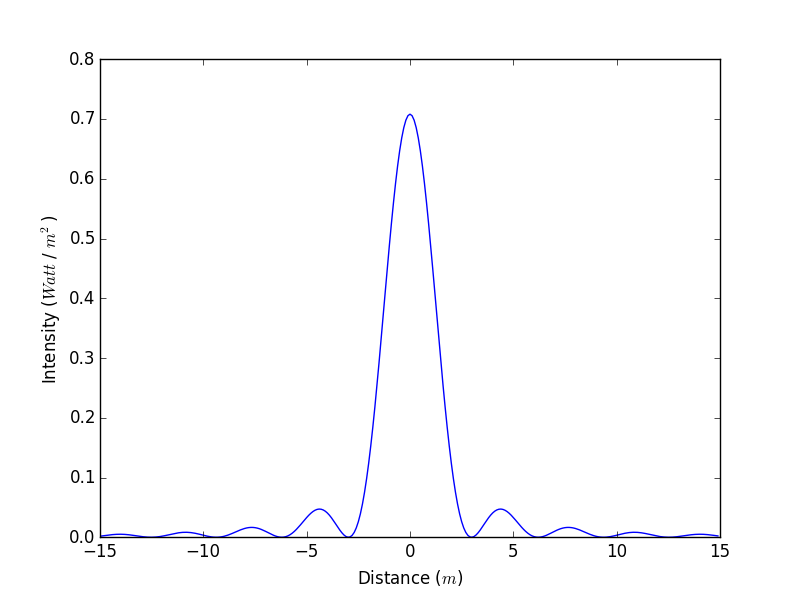
\includegraphics[scale=0.45]{figure_1.png}
\caption{Intensity (averaged on time) profile of single antenna}
\end{figure}

\begin{figure}[!h]
\centering	
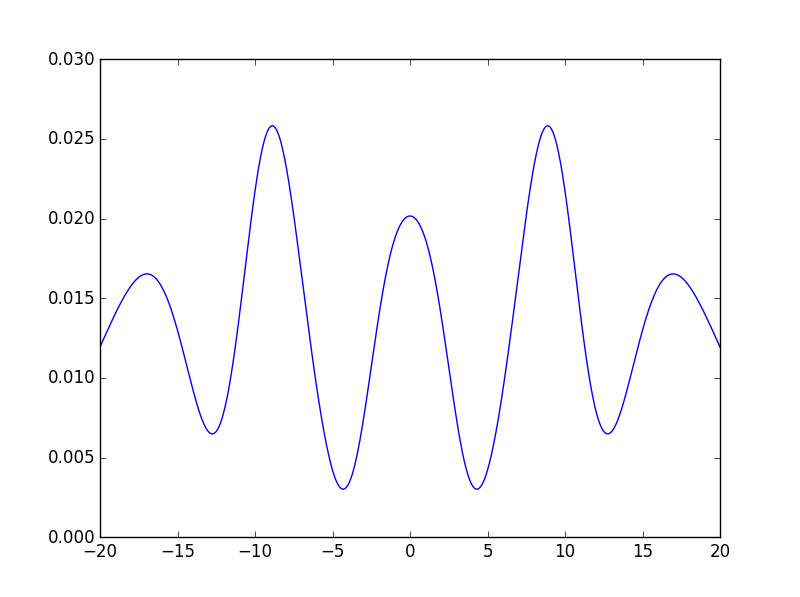
\includegraphics[scale=0.45]{figure_2.png}
\caption{Intensity (time averaged) profile of single antenna}
\end{figure}

\subsection{Discussion}

Here we have a single isotropic antenna source, radiating over a sphere centered on the source. We get Fig. (4.1) when we averaged the intensity of this single isotropic source over time and after averaging time we have Fig. (4.2) where the intensity decreases as the lateral distance increases as it should (according to the inverse square law), because we have a spherical wave moving radially. In the center of the screen we have maximum intensity because that is the closest point to the source. 


\section{Intensity of Linear Array of 4 Antennae}

Plot between distance and intensity, for four antenna sources arrange in a linear array, all of them being in phase. It is immediately obvious that we have an interference pattern. The relevant code can be found in appendix \ref{code:four}.

\begin{figure}[!h]
	\centering	
    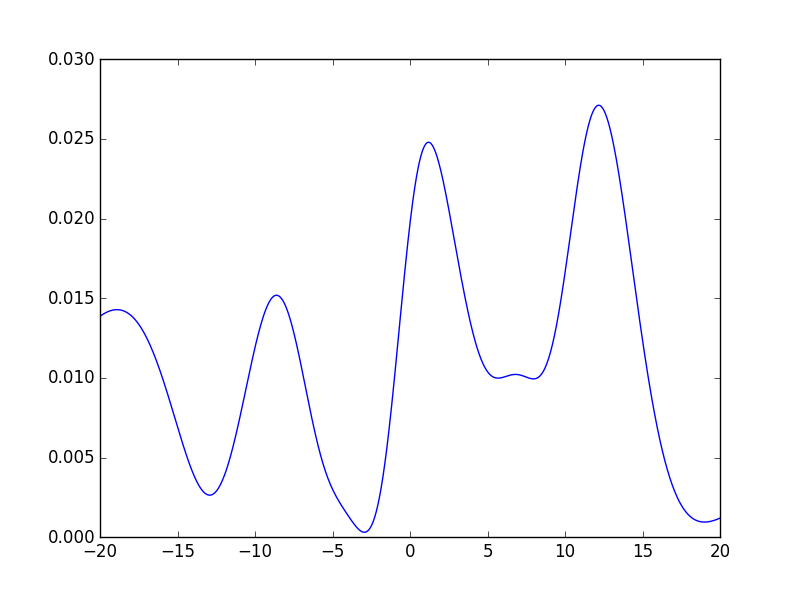
\includegraphics[scale=0.45]{figure_3.png}
	\caption{Intensity profile of linear array of 4 antennae}
\end{figure}

\subsection{Discussion}
We have 4 antenna sources arranged in a linear array. We get this radiation pattern by the contribution of all the antenna sources in the array. We get different lobes because of interference. Wherever spherical waves coming from each individual antenna source arrive in phase they add together (constructive interference) to enhance the intensity and where they arrive out of phase, with the peak of one coinciding with the another, the waves cancel (destructive interference) reducing the intensity in that direction.

\subsection{Managing Phase}

We used the same linear array of 4 antenna sources but modified the phase between them. Fig. (\ref{fig:phase_1}) (created using code \ref{code:phase_right}) corresponds to three antennas in phase and the right-most antenna completely out of phase ($\pi$ radians). Note how the intensity profile is no longer symmetric but in fact is shifting to the right. 

Fig. (\ref{fig:phase_2}) (created using code \ref{code:phase_left}) corresponds to the left-most antenna being completely out of phase while the remaining three are exactly in phase. The peak intensity shifts to the left. It is clear that by changing the phase we are steering the direction of peak intensity, that is, steering the beam.

\begin{figure}[!h]
	\centering	
	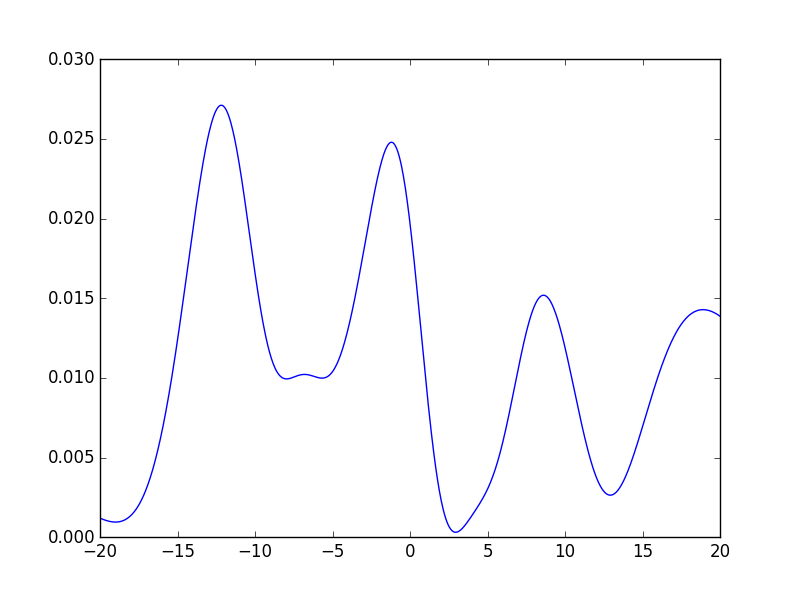
\includegraphics[scale=0.45]{figure_4.png}
    \caption{\label{fig:phase_1} Intensity profile of linear array of 4 antennae with 3 antennae in-phase and right-most antenna completely out of phase.}
\end{figure}

\begin{figure}[!h]
	\centering	
	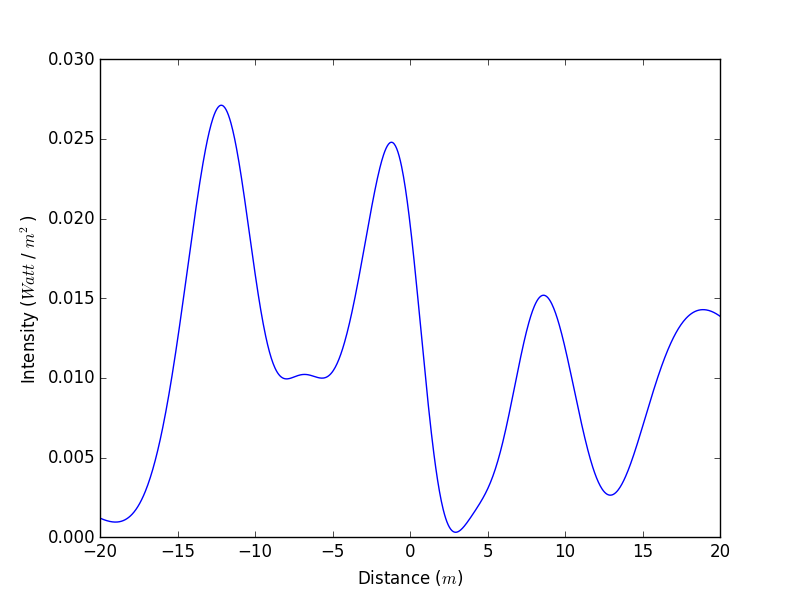
\includegraphics[scale=0.45]{figure_5.png}
    \caption{\label{fig:phase_2} Intensity profile of linear array of 4 antennae with 3 antennae in-phase and left-most antenna completely out of phase.}
\end{figure}

\subsubsection{Discussion}

These are the radiation patterns of interference between spherical waves produced with different phase between them. The result is a radiation pattern consisting of a strongly steered beam in one direction, plus a series of weaker beams, usually representing residual radiation in \textbf{unwanted} directions that can not participate in beam formation.

	
    \begin{appendices}
      \chapter{Python Code}

\section{Intensity vs. lateral distance for a single source}\label{code:single}

\begin{Verbatim}[fontsize=\small,baselinestretch=0.9]
import matplotlib.pyplot as plt
from math import sqrt, sin
w=1 #(t'=wt)
k=1 #(r'=kr)
L=1

% r(x) is the distance between the source and the point x on the screen from the center x=0.
def r(x):
   return sqrt(L**2+x**2)

% Ex(x,t) is the electric field component of the source along x-axis.
def Ex(x,t):
   return (x/r(x)**2)*(sin(k*r(x)-w*t))

% Ey(x,t) is the electric field component of the source along y-axis.
def Ey(x,t):
   return (L/r(x)**2)*(sin(k*r(x)-w*t))

% I(x,t) is the intensity for a single source.
def I(x,t):
   return (Ex(x,t)**2+Ey(x,t)**2)

#plot between intensity and distance.
a=[]
b=[]

for i in range(-150,150,1):
   x=i/10.0
   y=I(x,0)
   a.append(x)
   b.append(y)

fig= plt.figure()
axes=fig.add_subplot(111)
axes.plot(a,b)
plt.show()
\end{Verbatim}


\section{Intensity vs. lateral distance for a linear array of 4 antennae}\label{code:four}

\begin{Verbatim}[fontsize=\small,baselinestretch=0.9]
import numpy as np
import matplotlib.pyplot as plt
from math import sqrt, sin, pi

w=1.0
k=1.0
L=10.0 / k
P=0

# Calculate fringe spacing:
#d = 2 * 5           # Slit-spacing
#fs = 2 * pi * L / (k * d)
#print("Slit-spacing = {} produces fringe spacing = {}".format(d, fs))

# sources=[(distance,phase)]
sources = [(-12, 0), (-4,0), (4,0), (12,0)]

% r(x,d) is the distance between the sources and the point x on the screen, and d is the distance between sources.
def r(x,d):
   return sqrt(L**2+(x-d)**2)

% Ex(x,d,p,t) is the electric field component of the sources along x-axis. where, p is the phase.
def Ex(x,d,p,t):
   return ((x-d)/r(x,d)**2)*(sin(k*r(x,d)-w*t+p))

% Ey(x,d,p,t) is the electric field component of the sources along y-axis. where, p is the phase.
def Ey(x,d,p,t):
   return (L/r(x,d)**2)*(sin(k*r(x,d)-w*t+p))

% I(x,t) is the intensity for multiple sources.
def I(x,sources,t):

   Ox=0
   Oy=0

   for d, p in sources:

      Ox+=Ex(x,d,p,t)
      Oy+=Ey(x,d,p,t)

   return Ox**2+Oy**2

% Intensity vs. lateral distance for a linear array of 4 antennae.
def trapezoidal(f, a, b, n):

   h = float(b - a) / n
   s = 0.0
   s += f(a)/2.0

   for i in range(1, n):
      s += f(a + i*h)
      s += f(b)/2.0

   return s * h


xs=[]
ys=[]


for x in np.linspace(-20,20,1000):
   y = trapezoidal(lambda t: I(x,sources,t), -pi/w, pi/w, 100) / (2 * pi)

xs.append(x)
ys.append(y)

plt.plot(xs,ys)
plt.show()   
\end{Verbatim}

\subsection{Steer the beam by introducing and managing phase}

\subsubsection{Example 1}\label{code:phase_right}

\begin{Verbatim}[fontsize=\small,baselinestretch=0.9]
import numpy as np
import matplotlib.pyplot as plt
from math import sqrt, sin, pi

w=1.0
k=1.0
L=10.0 / k

#sources=[(distance,phase)]
sources = [(-12,0), (-4,0), (4,0), (12,pi)]

% r(x,d) is the distance between the sources and the point x on the screen, and d is the distance between sources.
def r(x,d):
    return sqrt(L**2+(x-d)**2)
    
% Ex(x,d,p,t) is the electric field component of the sources along x-axis. where, p is the phase.
def Ex(x,d,P,t):
    return ((x-d)/r(x,d)**2)*(sin(k*r(x,d)-w*t+P))

% Ey(x,d,p,t) is the electric field component of the sources along y-axis. where, p is the phase.
def Ey(x,d,P,t):
    return (L/r(x,d)**2)*(sin(k*r(x,d)-w*t+P))
       
% I(x,t) is the intensity for multiple sources.
def I(x,sources,t):
    Ox=0
    Oy=0
    for d, p in sources:
        Ox+=Ex(x,d,p,t)
        Oy+=Ey(x,d,p,t)
    
    return Ox**2+Oy**2
        
% Intensity vs. lateral distance for a linear array of 4 antennae by managing phase.
def trapezoidal(f, a, b, n):
    h = float(b - a) / n
    s = 0.0
    s += f(a)/2.0
    for i in range(1, n):
        s += f(a + i*h)
    s += f(b)/2.0
    return s * h

xs=[]
ys=[]

for x in np.linspace(-20,20,1000):
    y = trapezoidal(lambda t: I(x,sources,t), -pi/w, pi/w, 100) / (2 * pi)
   
    xs.append(x)
    ys.append(y)

plt.plot(xs,ys)
plt.show()   
\end{Verbatim}


\subsubsection{Example 2}\label{code:phase_left}

\begin{Verbatim}[fontsize=\small,baselinestretch=0.9]
import numpy as np
import matplotlib.pyplot as plt
from math import sqrt, sin, pi

w=1.0
k=1.0
L=10.0 / k

#sources=[(distance,phase)]
sources = [(-12,0), (-4,pi), (4,pi), (12,pi)]

% r(x,d) is the distance between the sources and the point x on the screen, and d is the distance between sources.
def r(x,d):
    return sqrt(L**2+(x-d)**2)
    
% Ex(x,d,p,t) is the electric field component of the sources along x-axis. where, p is the phase.
def Ex(x,d,P,t):
    return ((x-d)/r(x,d)**2)*(sin(k*r(x,d)-w*t+P))
   
% Ey(x,d,p,t) is the electric field component of the sources along y-axis. where, p is the phase.
def Ey(x,d,P,t):
    return (L/r(x,d)**2)*(sin(k*r(x,d)-w*t+P))
 
% I(x,t) is the intensity for multiple sources.
def I(x,sources,t):
    Ox=0
    Oy=0
    for d, p in sources:
        Ox+=Ex(x,d,p,t)
        Oy+=Ey(x,d,p,t)
    
    return Ox**2+Oy**2
        
% Intensity vs. lateral distance for a linear array of 4 antennae by managing phase.
def trapezoidal(f, a, b, n):
    h = float(b - a) / n
    s = 0.0
    s += f(a)/2.0
    for i in range(1, n):
        s += f(a + i*h)
    s += f(b)/2.0
    return s * h

xs=[]
ys=[]

for x in np.linspace(-20,20,1000):
    y = trapezoidal(lambda t: I(x,sources,t), -pi/w, pi/w, 100) / (2 * pi)
   
    xs.append(x)
    ys.append(y)

plt.plot(xs,ys)
plt.show()
\end{Verbatim}

    \end{appendices}
	
	\makereferences         % Create the references section
	
\end{document}


